\chapter{Performances of Different Numerical Methods}
\label{chapter5}

In this chapter, we will see some 

\section{The CSR Method: Limitations and Usability}
The CSR method, described in section~\ref{chapter3_csr}, has been studied and implemented in order to analyze the model described in the last section. The algorithm is written in pseudocode in appendix~\ref{AppendixA}.

In this section, it is shown that the CSR method is not a suitable method for investigating systems described by a model such as the one under consideration.

In order to reveal this, we can easily see the case of a 4-sites chain for the proposed model. In particular, we can study the magnetization profile of the chain, i.e. the steady-state expectation value $\langle \sigma^z \rangle$ of the Pauli spin- matrix $\sigma^z$ for each site:
\begin{equation*}
    \langle \sigma^z \rangle = \Tr(\sigma^z \rho),
\end{equation*}
being $\rho$ the steady-state density matrix of the system.

\begin{figure}[H]
    \centering
    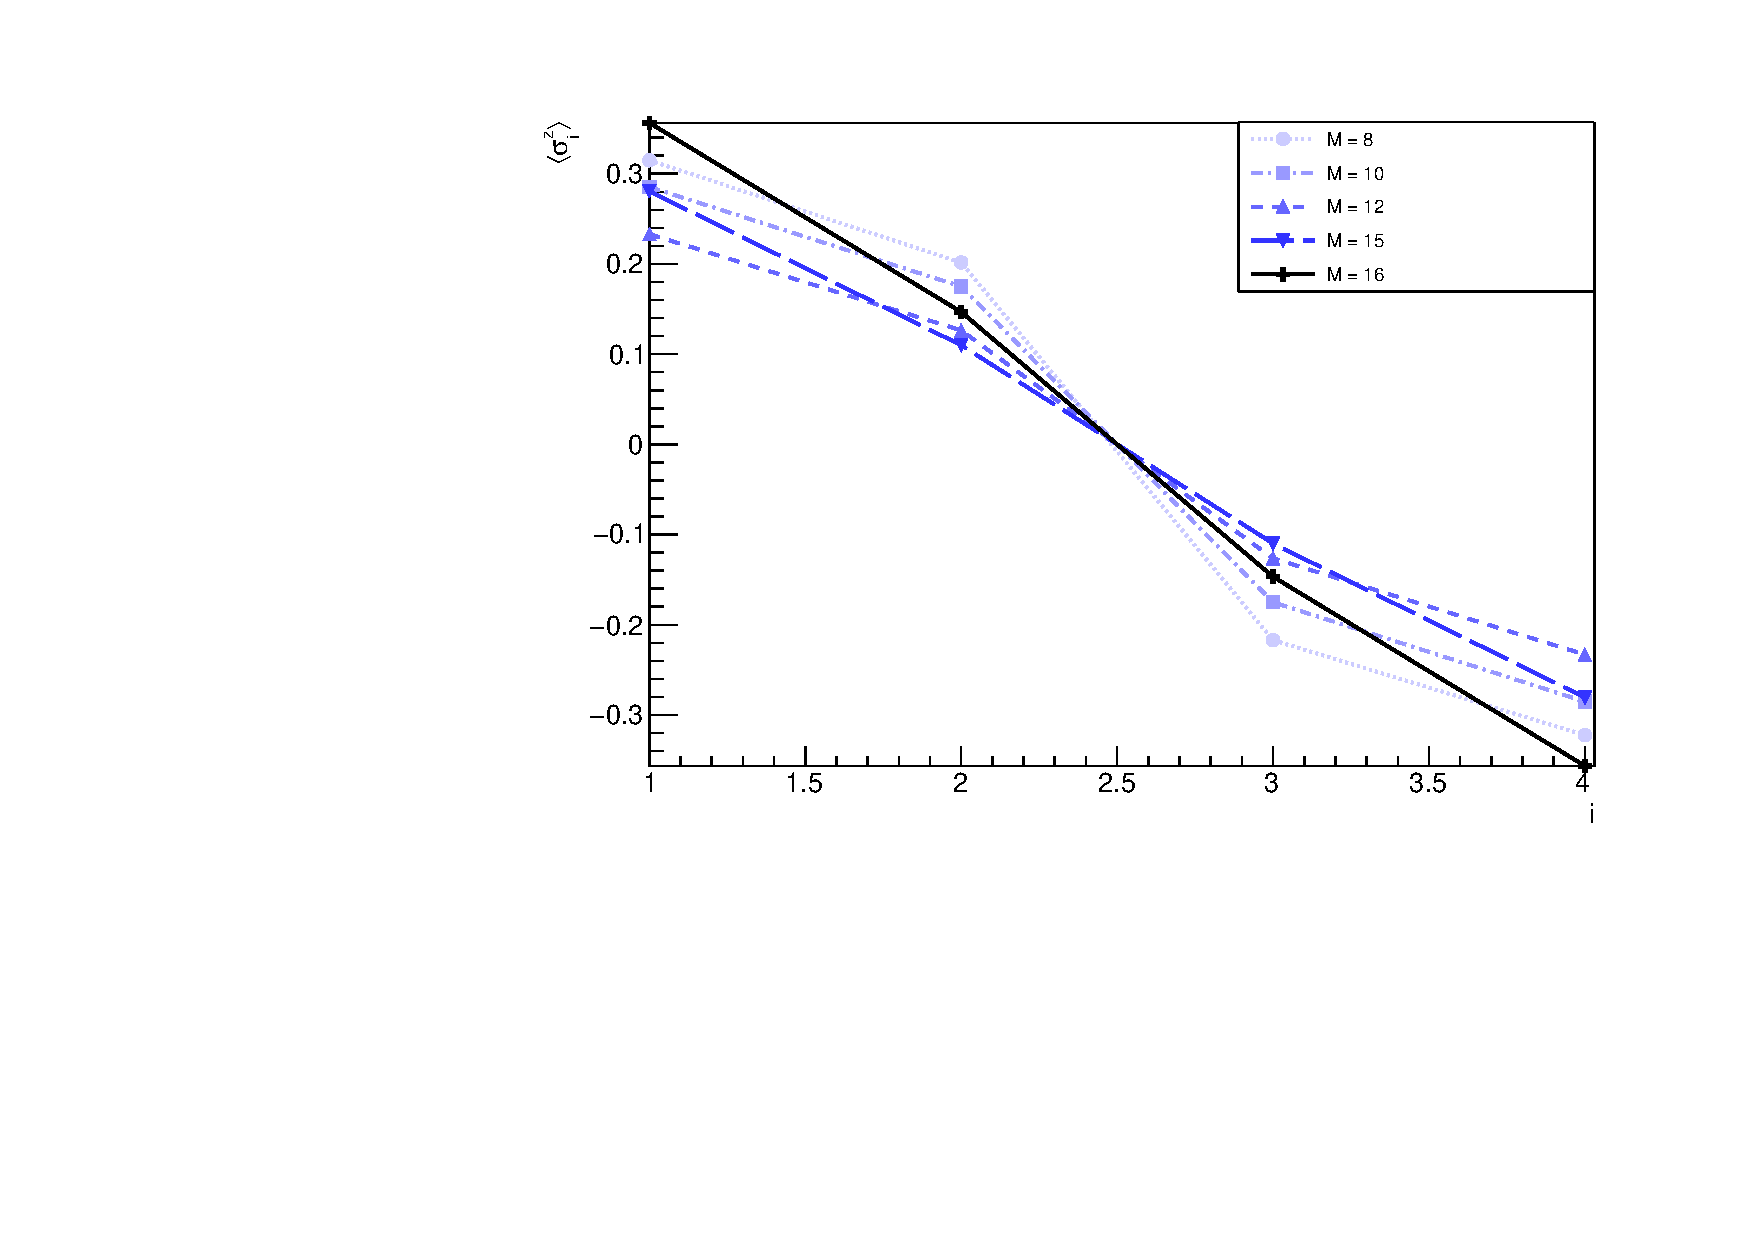
\includegraphics[scale=0.7]{Figures/4sites/4sites_LM_convergenceIncreasingM.pdf}
    \captionsetup{width=1.\linewidth}
    \caption{Spin profile of a 4-sites chain for the model described above with $J_z=1$ for several values of corner-space dimensions $M \times M$. The cyan markers are those representing the expectation value of the magnetization calculated by means of a complete set of states of Hilbert space (which has dimension $2^4$).}
    \label{fig:4sites_LM_convergenceIncreasingM}
\end{figure}

As shown in figure~\ref{fig:4sites_LM_convergenceIncreasingM}, it is clear that for such a system the convergence has not been reached. Even for $M = 15$, that covers almost the total Hilbert space dimension, the results are not the convergent ones.

On the other hand, if we consider a model in which every site is coupled to a dissipator, we can see how the magnetization profile gets to convergence starting from $M = 9$ already.


\begin{figure}[H]
    \centering
    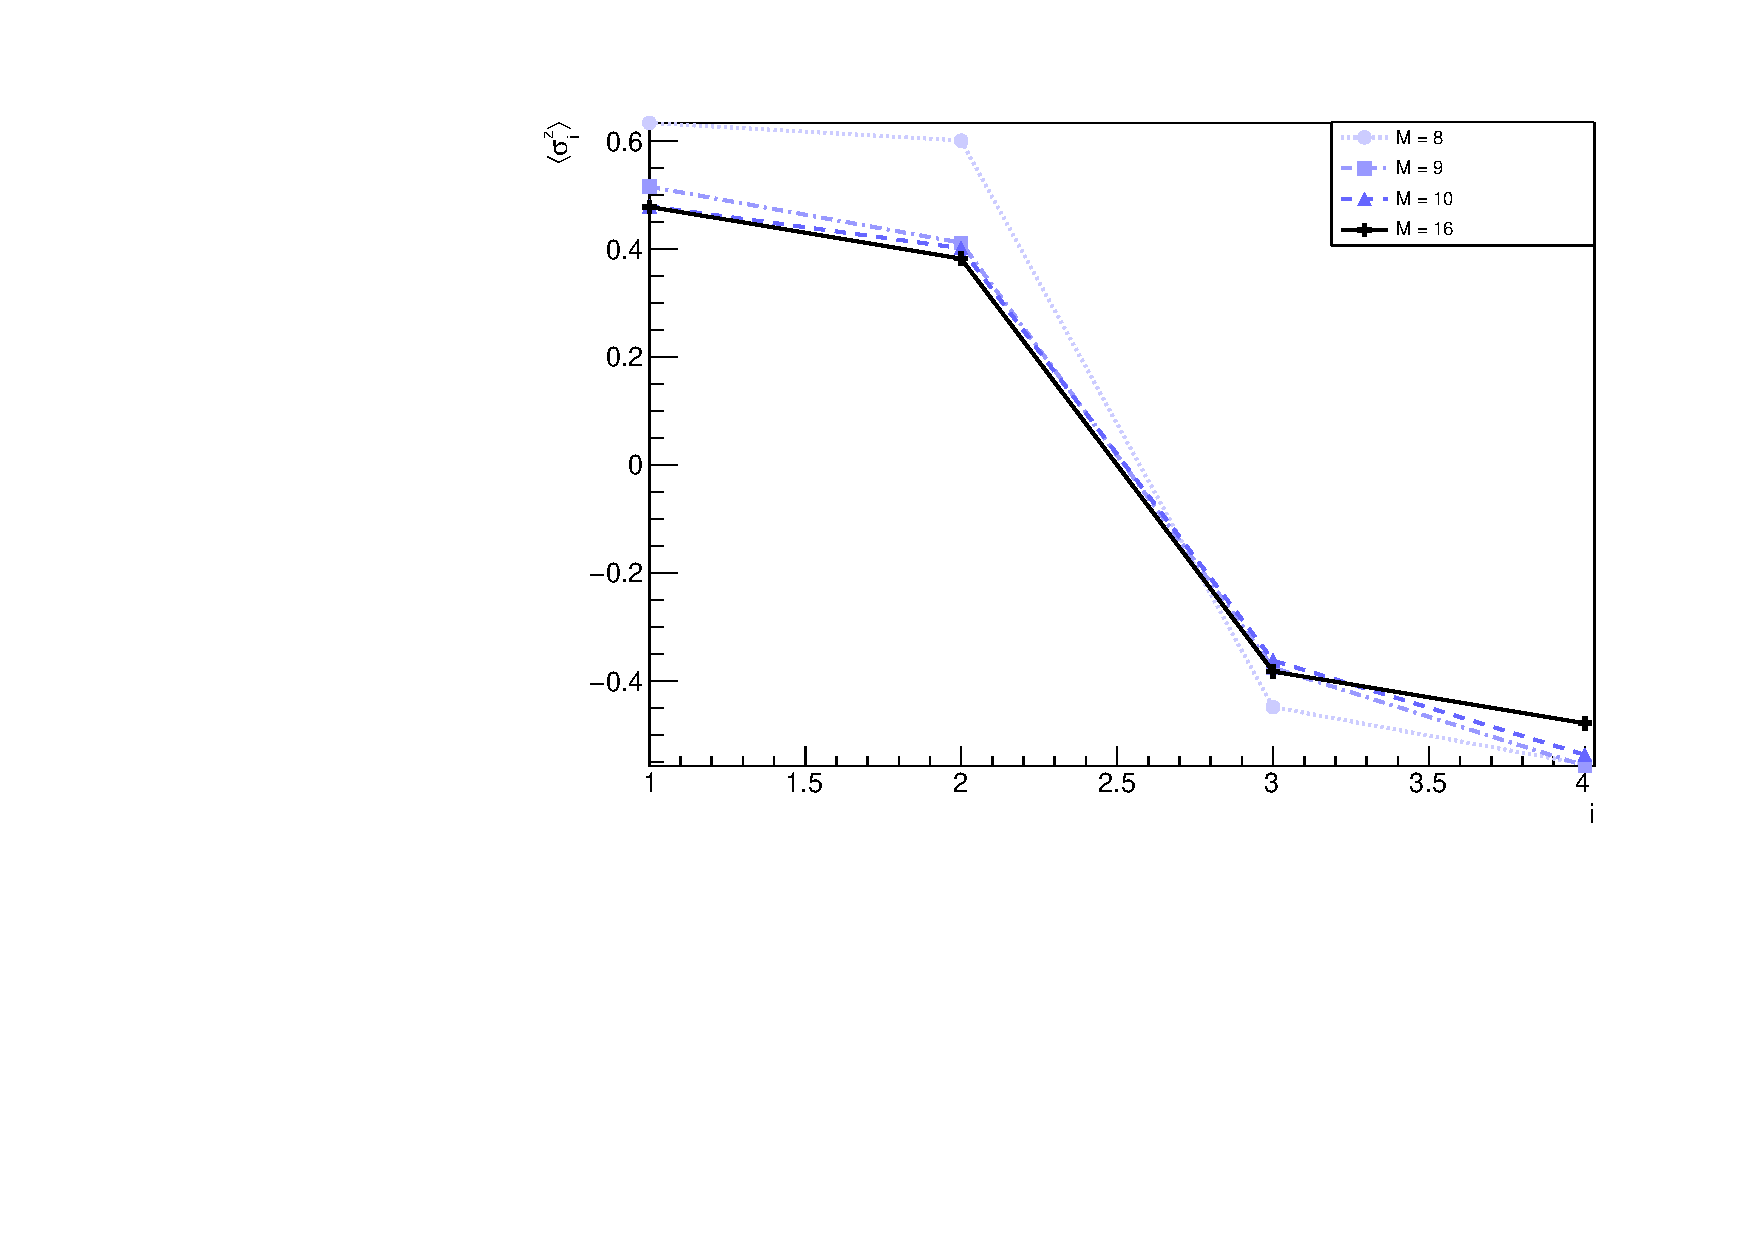
\includegraphics[scale=0.7]{Figures/4sites/4sites_totalDissipators.pdf}
    \captionsetup{width=1.\linewidth}
    \caption{Spin profile of a 4-sites chain in which every spin of the chain is coupled to a dissipator. In this case, the convergence is reached for $M<\text{dim}(\mathcal{H})$.}
    \label{fig:4sites_totalDissipators}
\end{figure}

In order to confirm the limitations of this method, the same comparison is done for a longer chain, made up by 8 sites. In this case, the results of CSR method are compared to those of MPO method, since a brute-force diagonalization of the Liouvillian operator would not be possible: it would require a huge amount of memory. We have reason to believe that the results obtained from MPO method are plausible, as we will see in the next sections.

\begin{figure}[H]
    \centering
    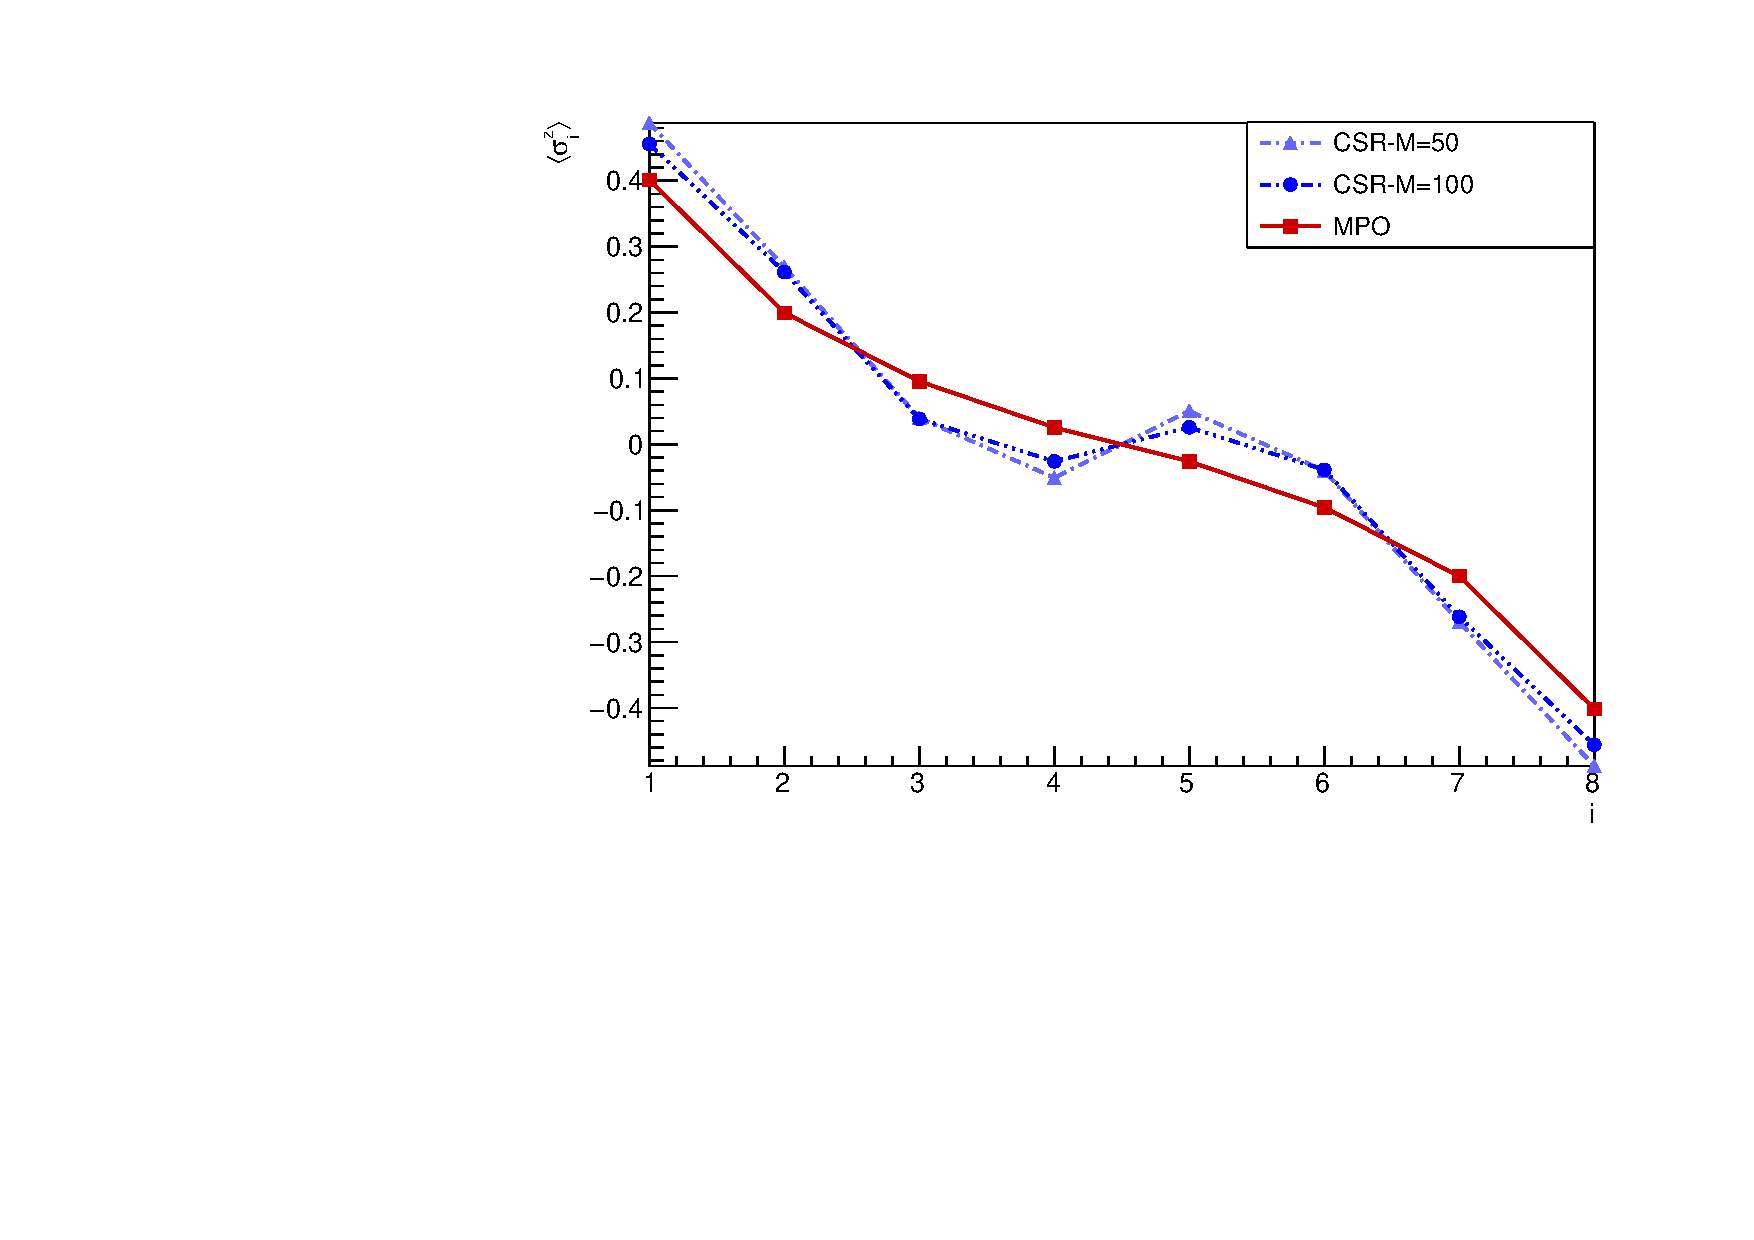
\includegraphics[scale=0.7]{Figures/8sites/1U1D_comparisonCSR_MPO_8site.pdf}
    \captionsetup{width=1.\linewidth}
    \caption{Spin profile of a 8-sites chain for the model described in sec.\ref{sec:model}. Significant differences between the data obtained for $M=50$ and $M=100$ are not noticed.}
    \label{fig:1U1D_comparisonCSR_MPO_8site}
\end{figure}

\begin{figure}[H]
    \centering
    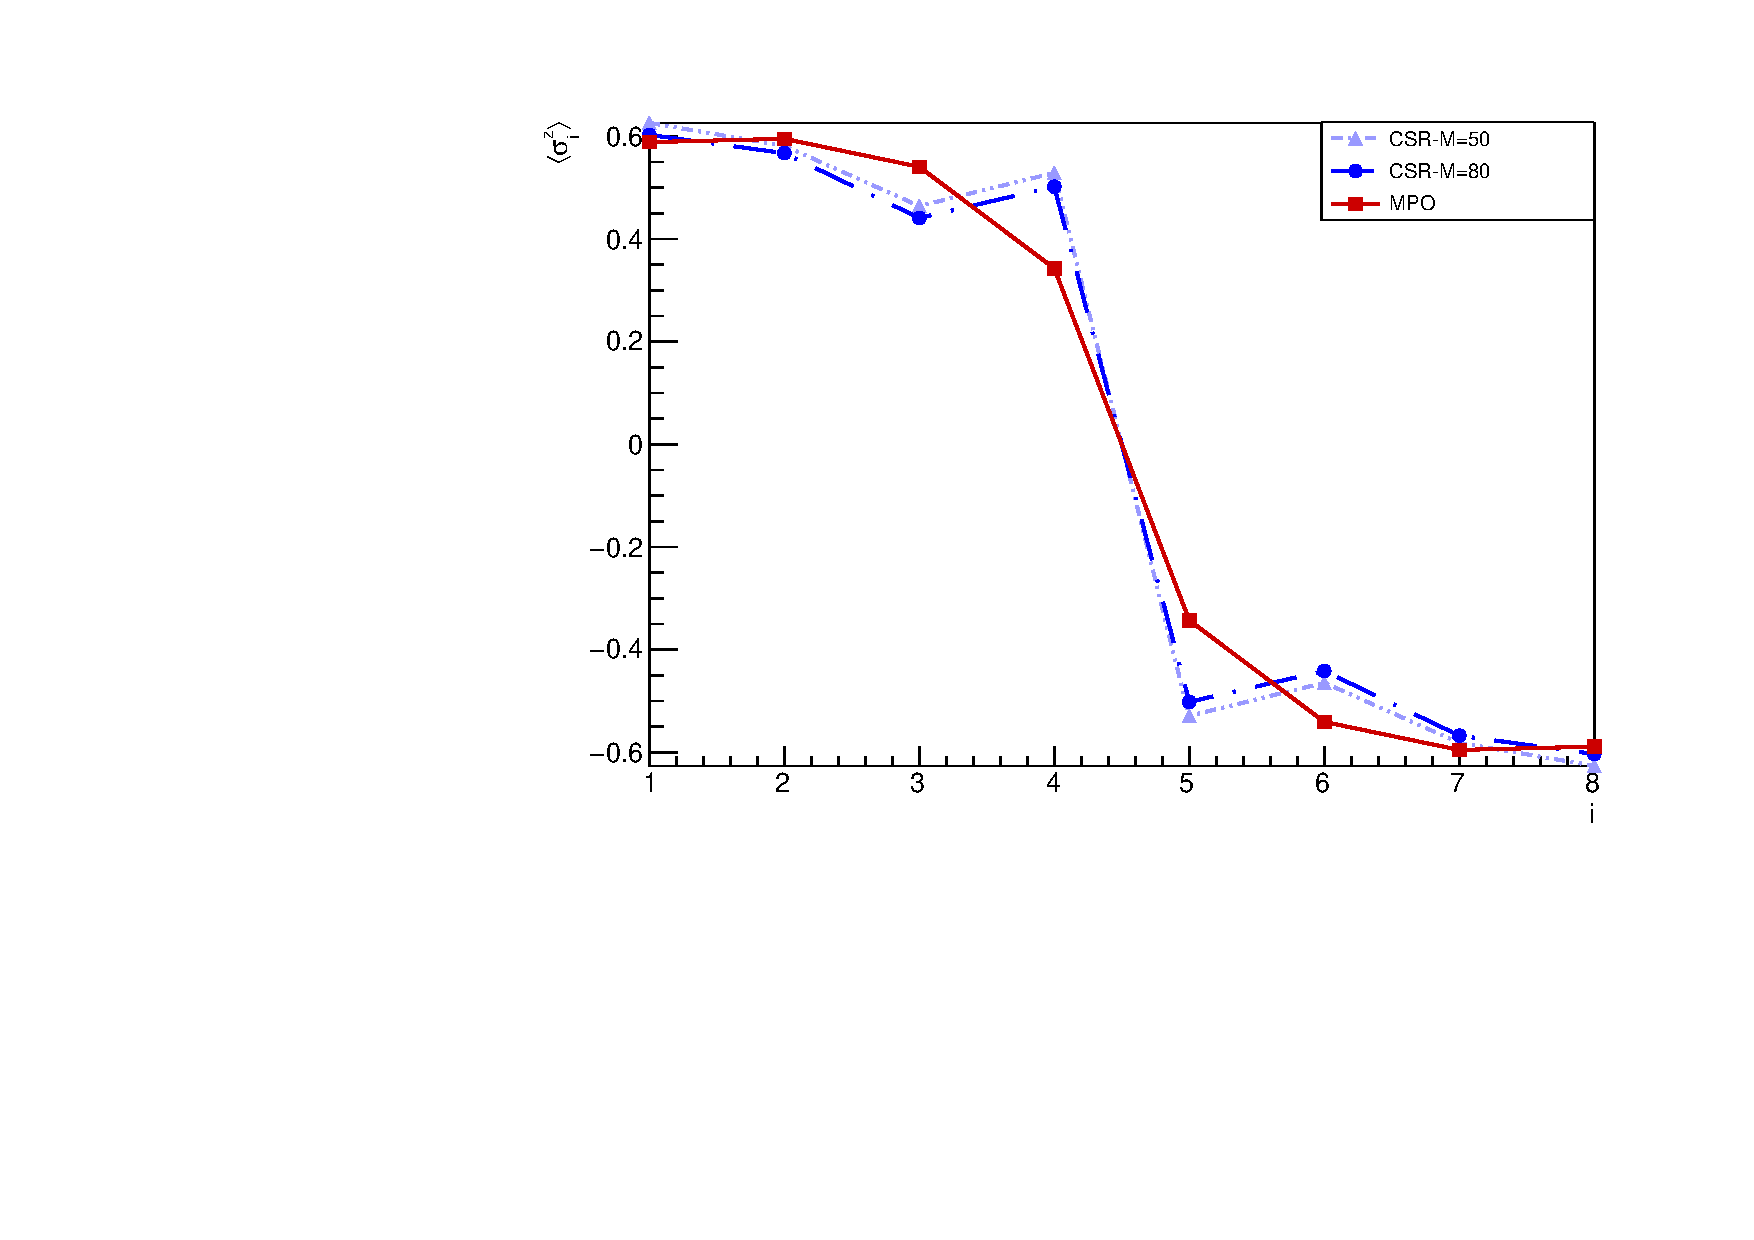
\includegraphics[scale=0.7]{Figures/8sites/8sites_MPOvsCORNER_4U4D.pdf}
    \captionsetup{width=1.\linewidth}
    \caption{Spin profile of a 8-sites chain in which every spin of the chain is coupled to a dissipator.}
    \label{fig:8sites_MPOvsCORNER_4U4D}
\end{figure}

In conclusion, in fig.~\ref{fig:LMComparison16s1051} it is displayed the magnetization profile of a 16-sites chain obtained by CSR and MPO methods.

\begin{figure}[H]
    \centering
    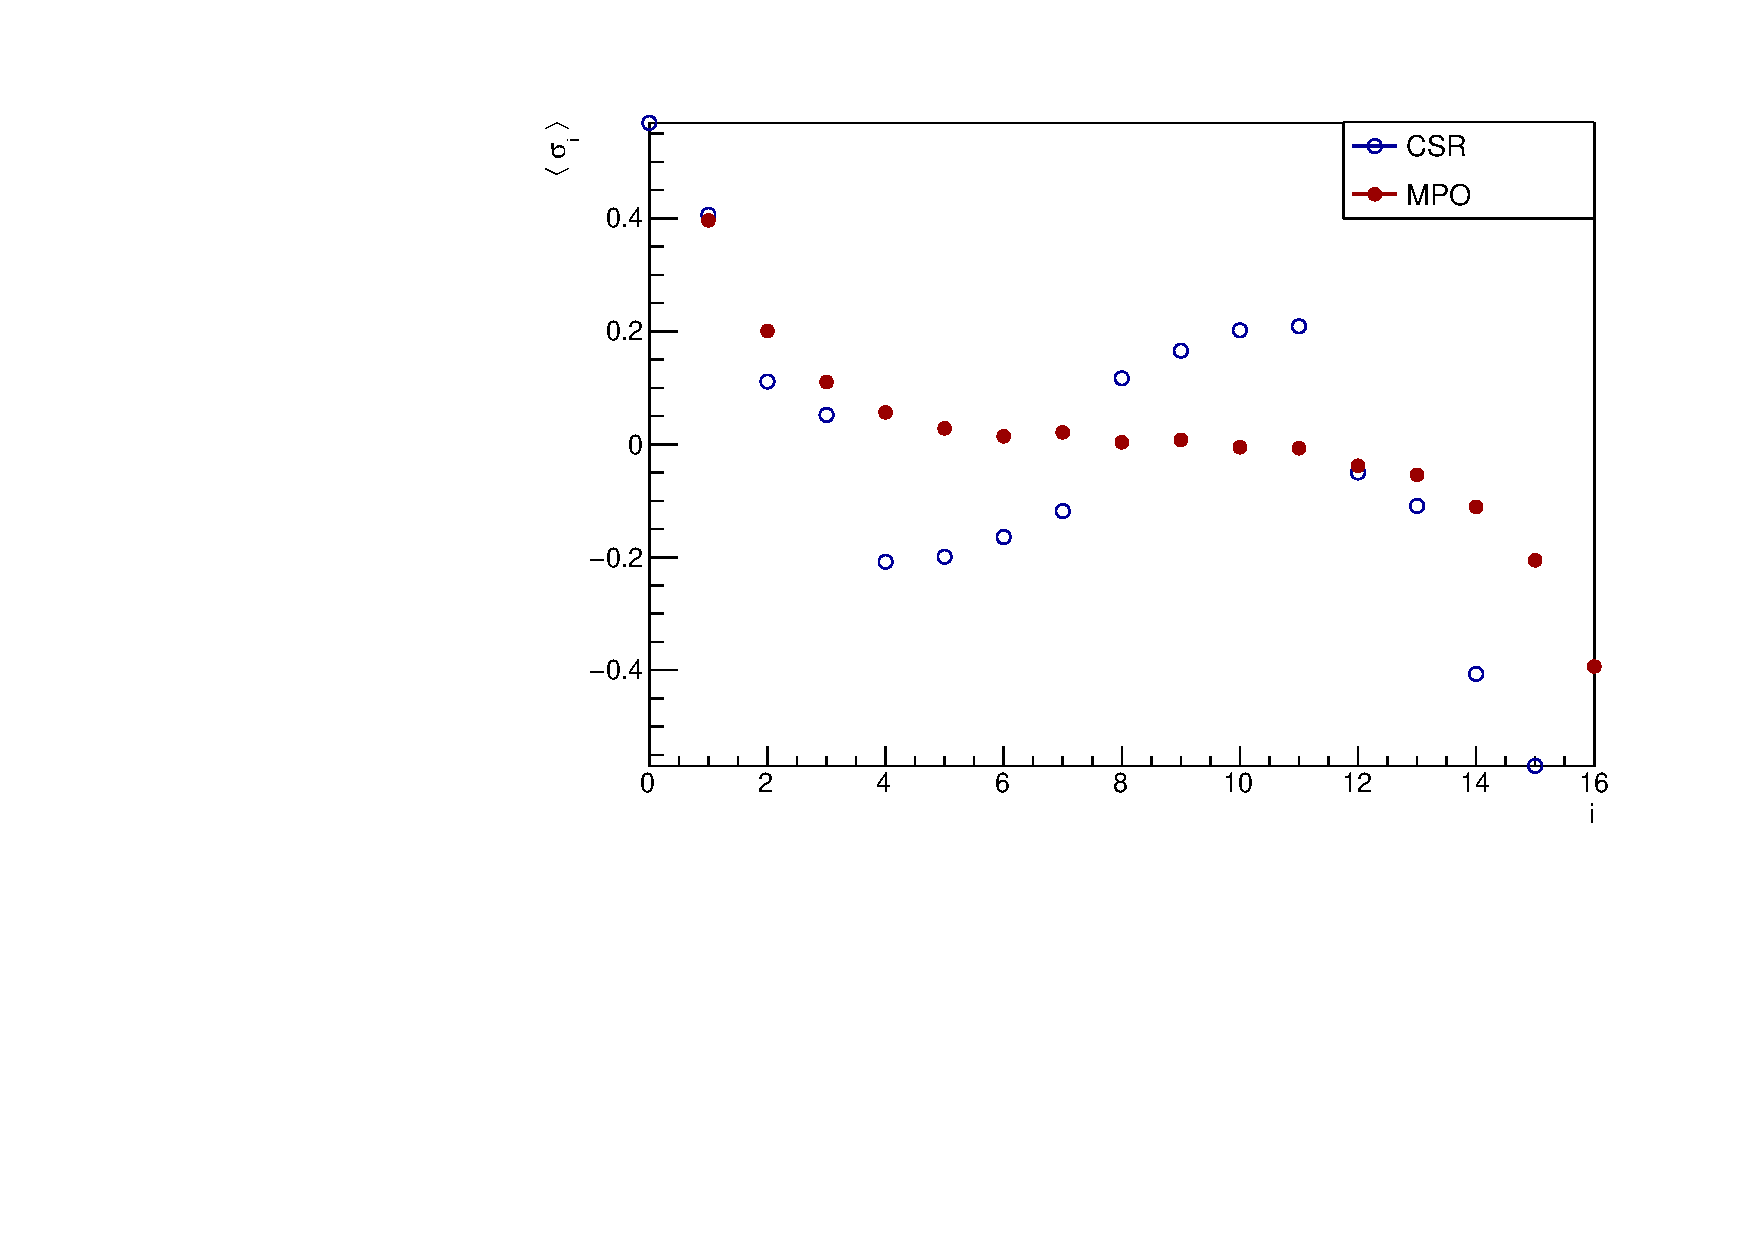
\includegraphics[scale=0.7]{Figures/16sites/LMComparison16s1051.pdf}
    \captionsetup{width=1.\linewidth}
    \caption{Spin profile for a 16-sites chain for the model described in section~\ref{sec:model}. Data in red are obtained from MPO method, with m = 80 and T = 2000 and data in blue are obtained from CSR method, with M = 65. It is self-evident the inadequacy of the corner-space method, for the model under study.}
    \label{fig:LMComparison16s1051}
\end{figure}

\begin{figure}[H]
    \centering
    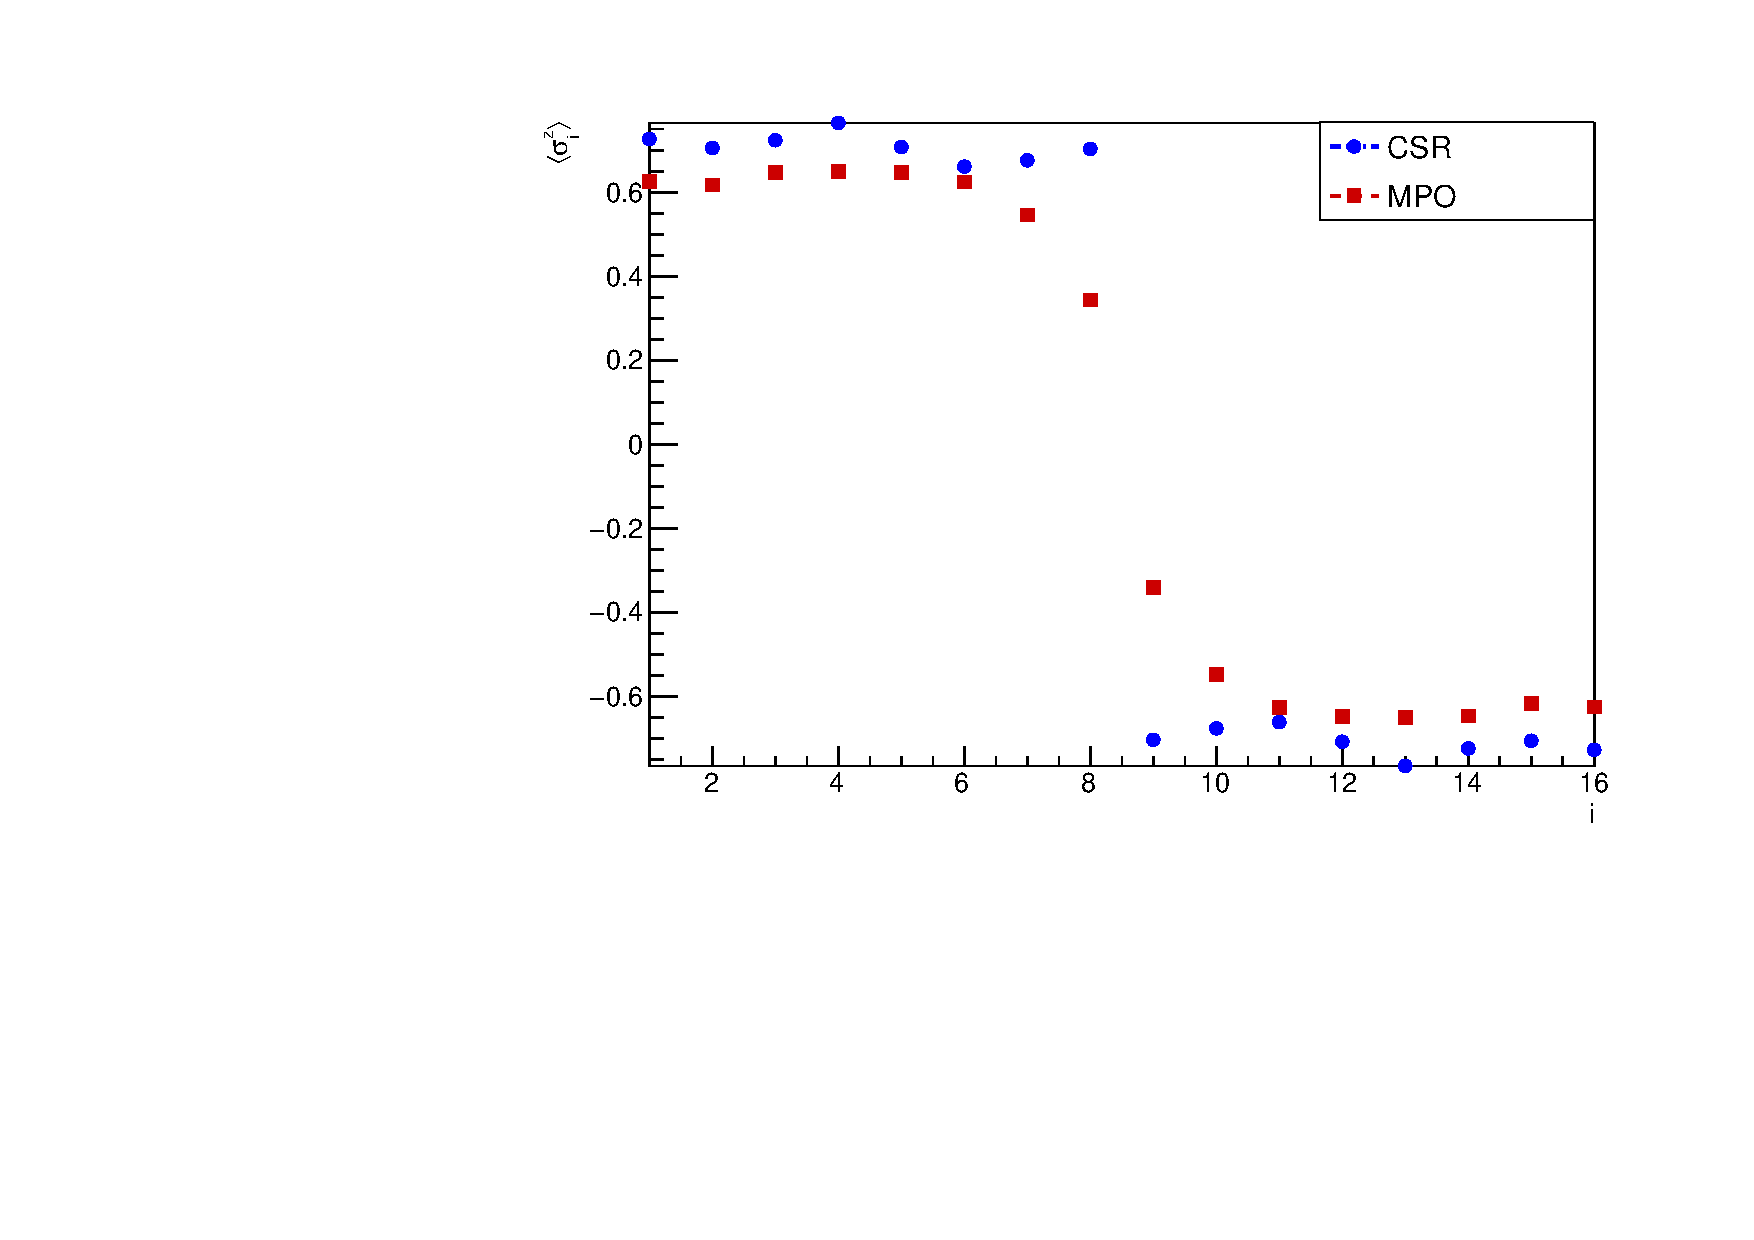
\includegraphics[scale=0.7]{Figures/8U8D_comparisonCSRvsMPO.pdf}
    \captionsetup{width=1.\linewidth}
    \caption{Spin profile for a 16-sites chain in which every spin of the chain is coupled to a dissipator. The dimension of the corner-space is $M=65$.}
    \label{fig:LMComparison16s1051}
\end{figure}

\section{Comparison between QT and MPO}
As a verification of the plausibility of data obtained from MPO method, we present here a comparison between the data obtained from MPO method and those obtained from QT method.

\begin{figure}
    \centering
        \begin{subfigure}{\columnwidth}
        \centering
        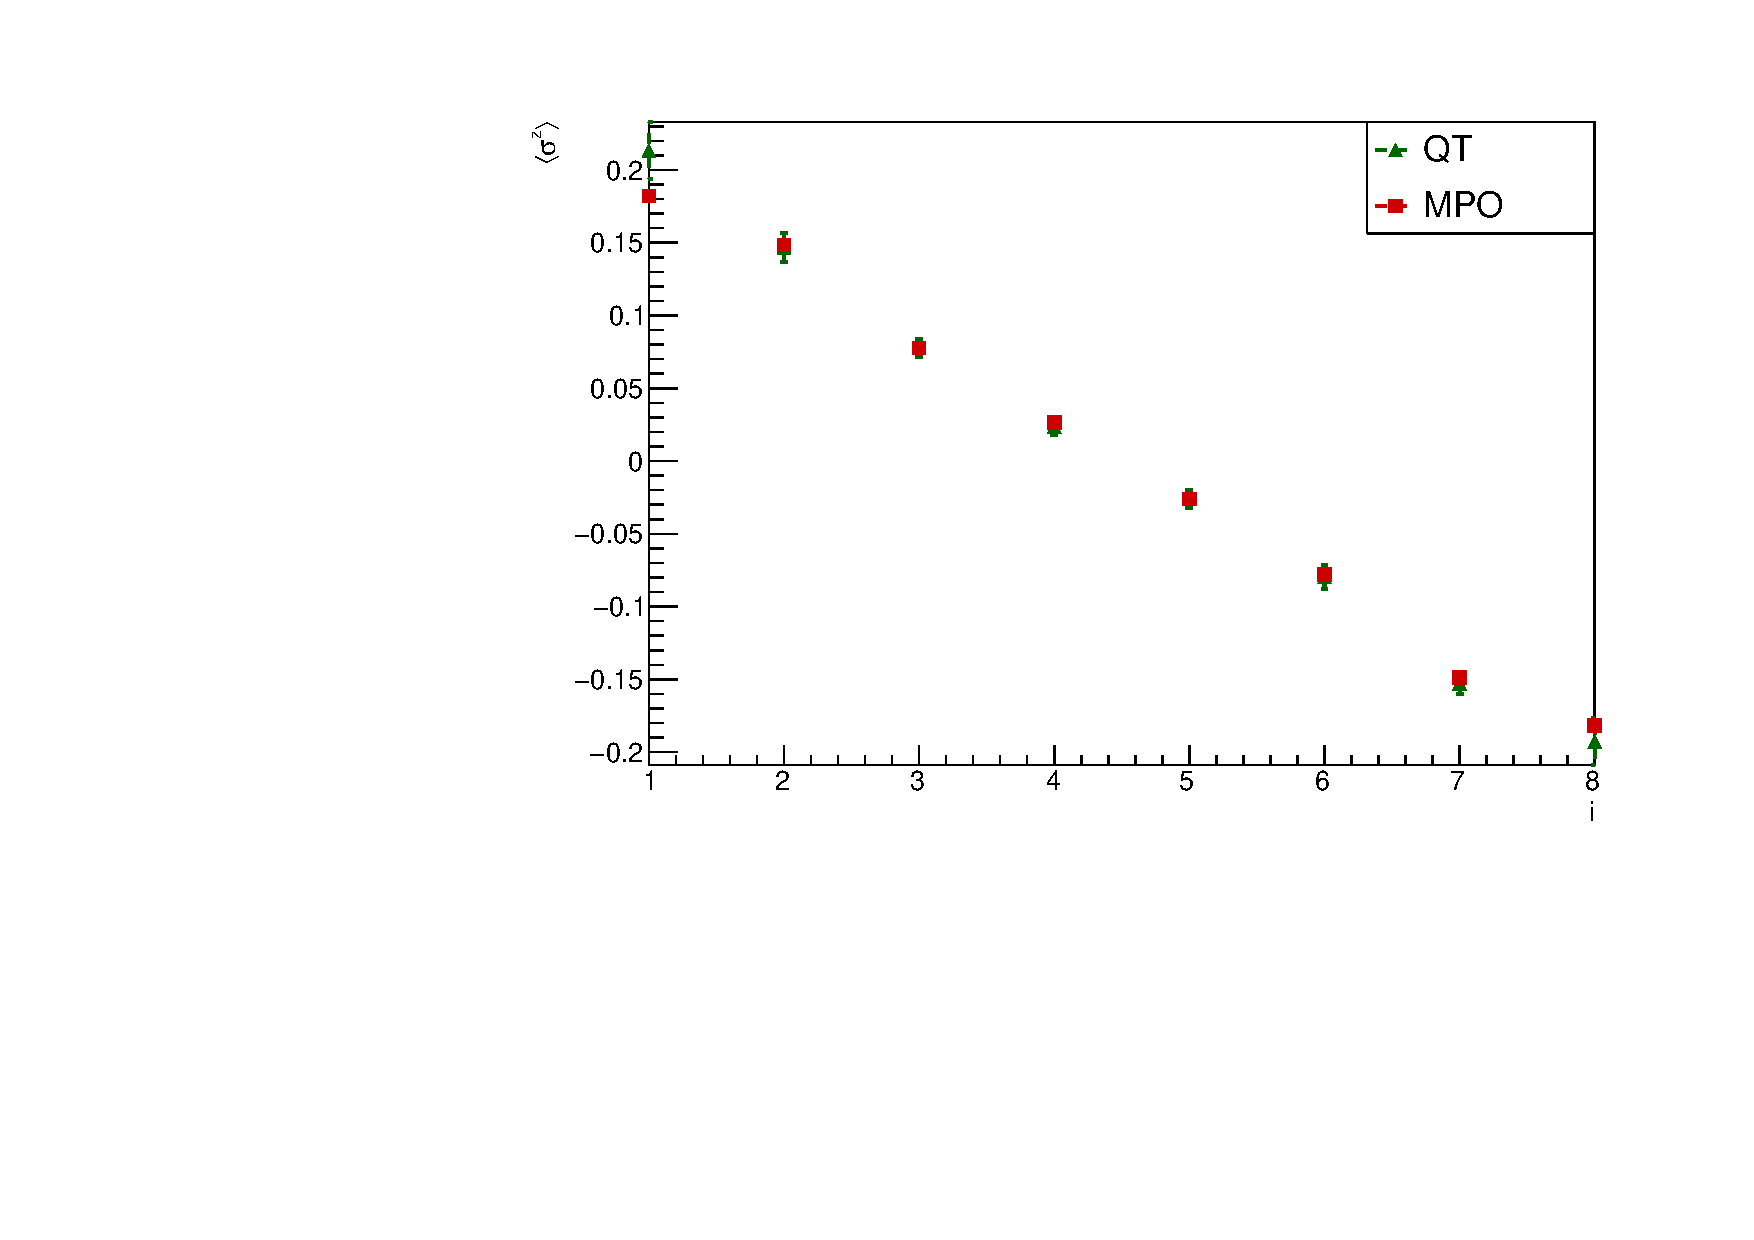
\includegraphics[scale=0.5]{Figures/LMComparison_8sJ10505.pdf}
        \label{fig:LMComparison_8sJ10505}
        \end{subfigure}\\
        \begin{subfigure}{\columnwidth}
        \centering
        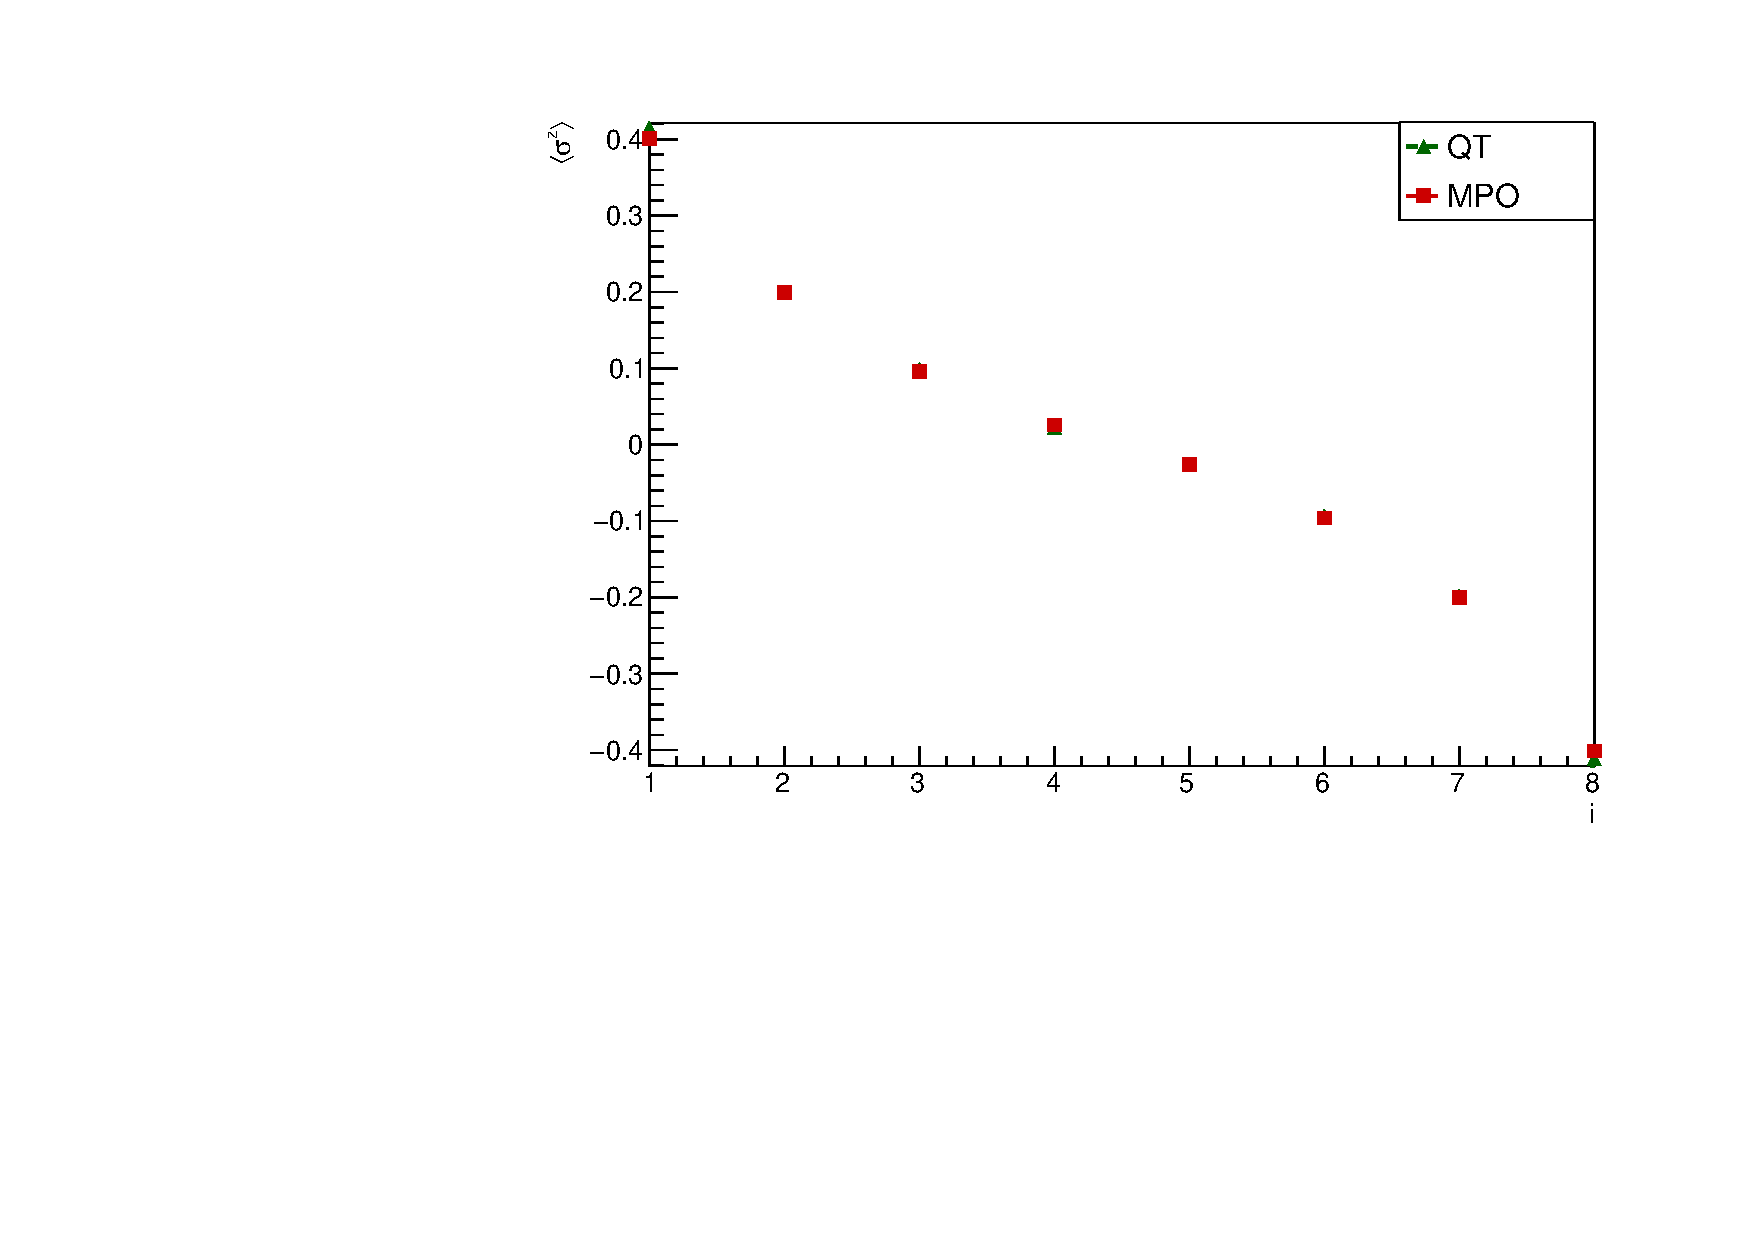
\includegraphics[scale=0.5]{Figures/LMComparison_8sJ1051.pdf}
        \label{fig:LMComparison_8sJ1051}
        \end{subfigure}\\
        \begin{subfigure}{\columnwidth}
        \centering
        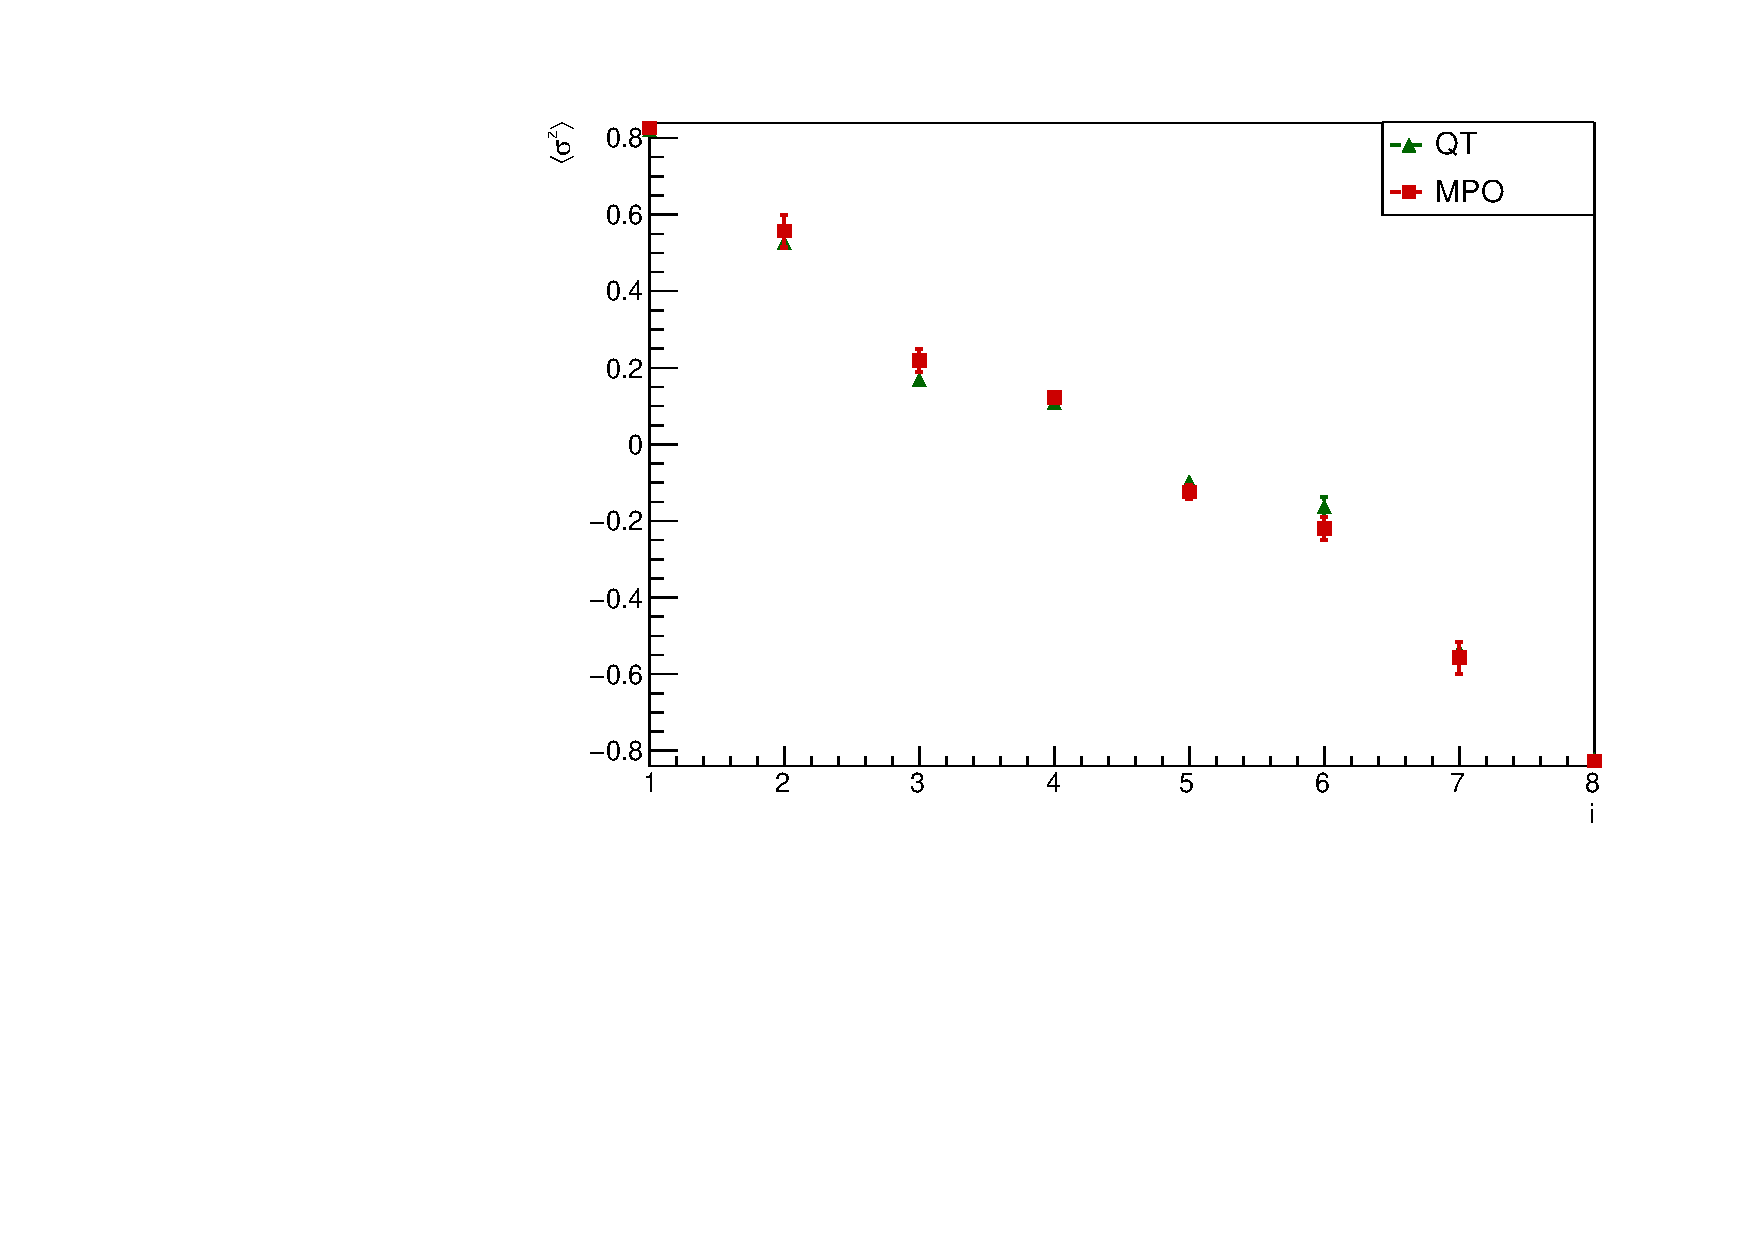
\includegraphics[scale=0.5]{Figures/LMComparison_8sJ10515.pdf}
        \label{fig:LMComparison_8sJ10515}
        \end{subfigure}\\
    \caption{Caption}
    \label{fig:my_label}
\end{figure}


\begin{figure}
    \centering
        \begin{subfigure}{\columnwidth}
        \centering
        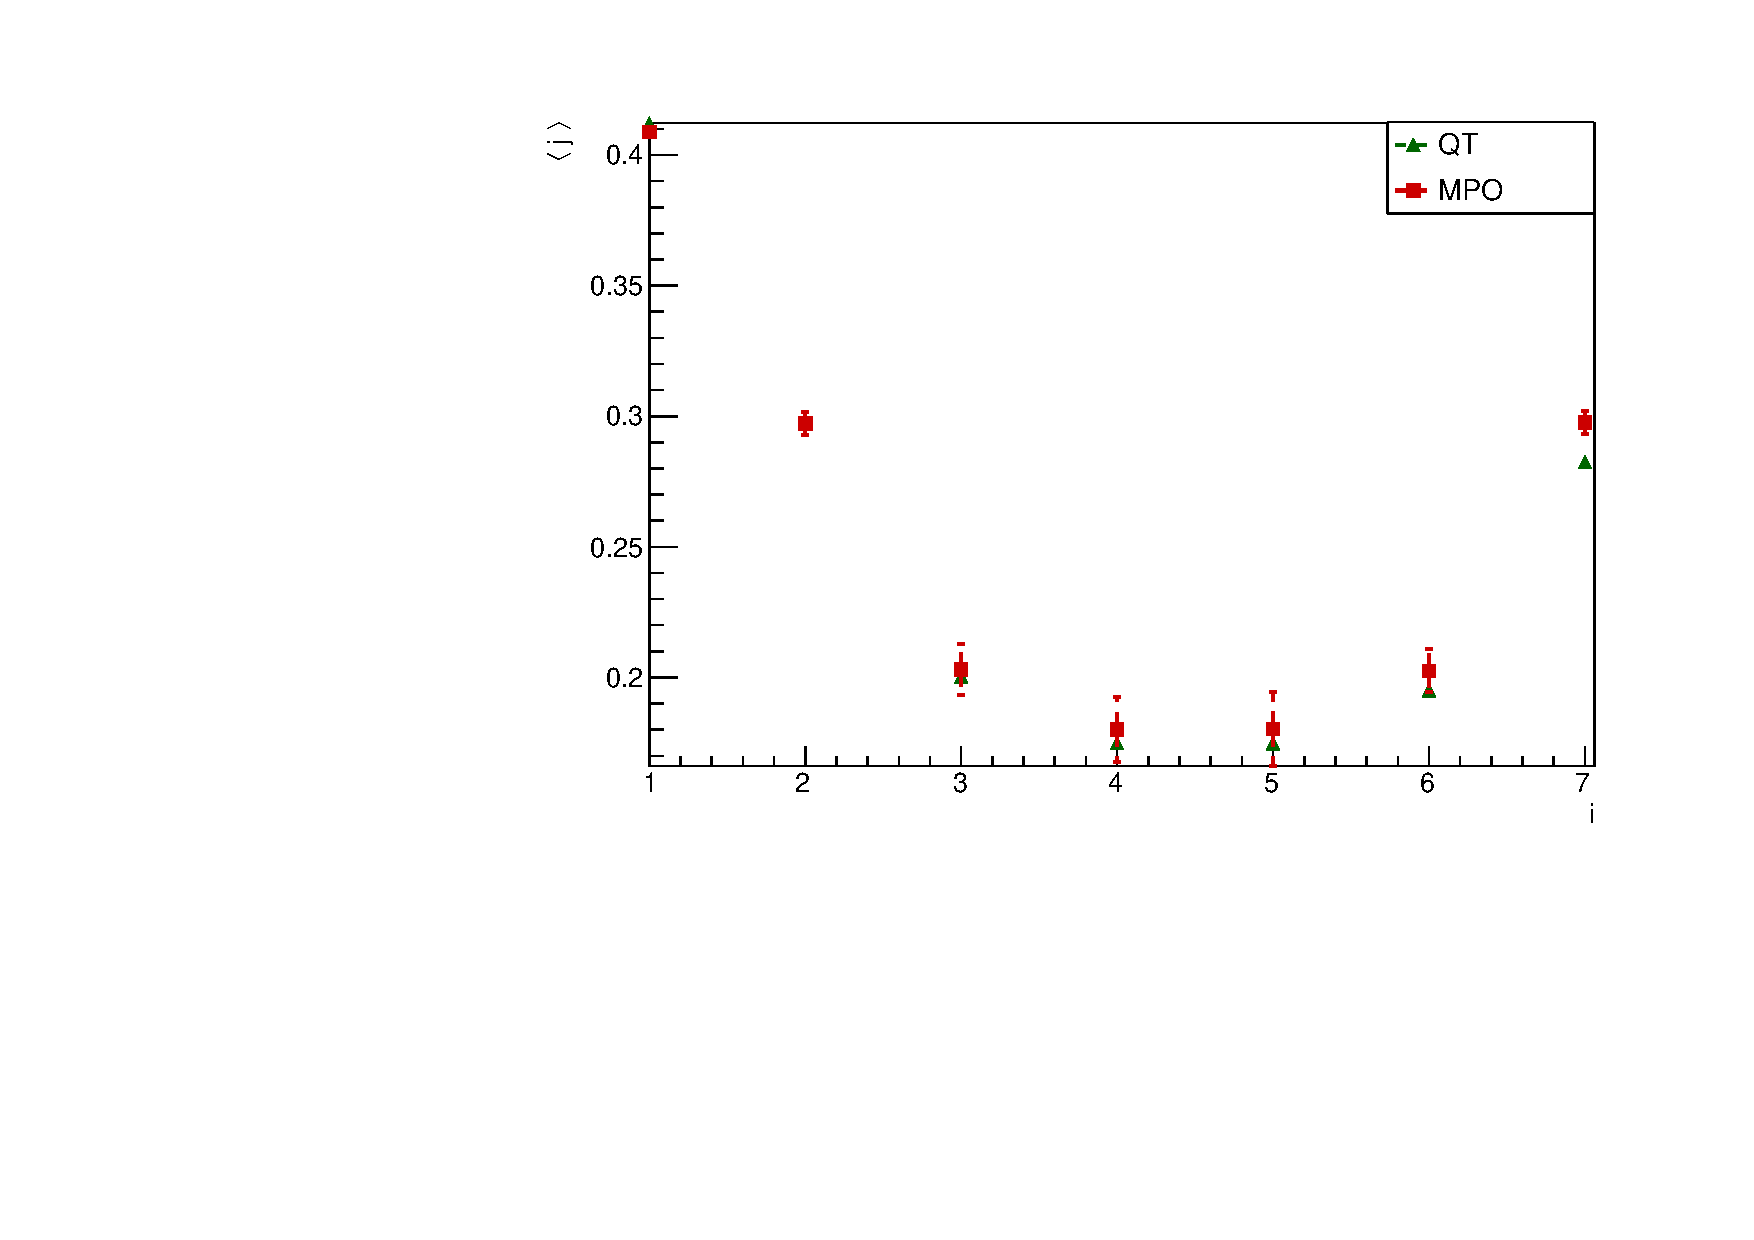
\includegraphics[scale=0.5]{Figures/SpinCurrComparison_8sJ10505.pdf}
        \label{fig:SpinCurrComparison_8sJ10505}
        \end{subfigure}\\
        \begin{subfigure}{\columnwidth}
        \centering
        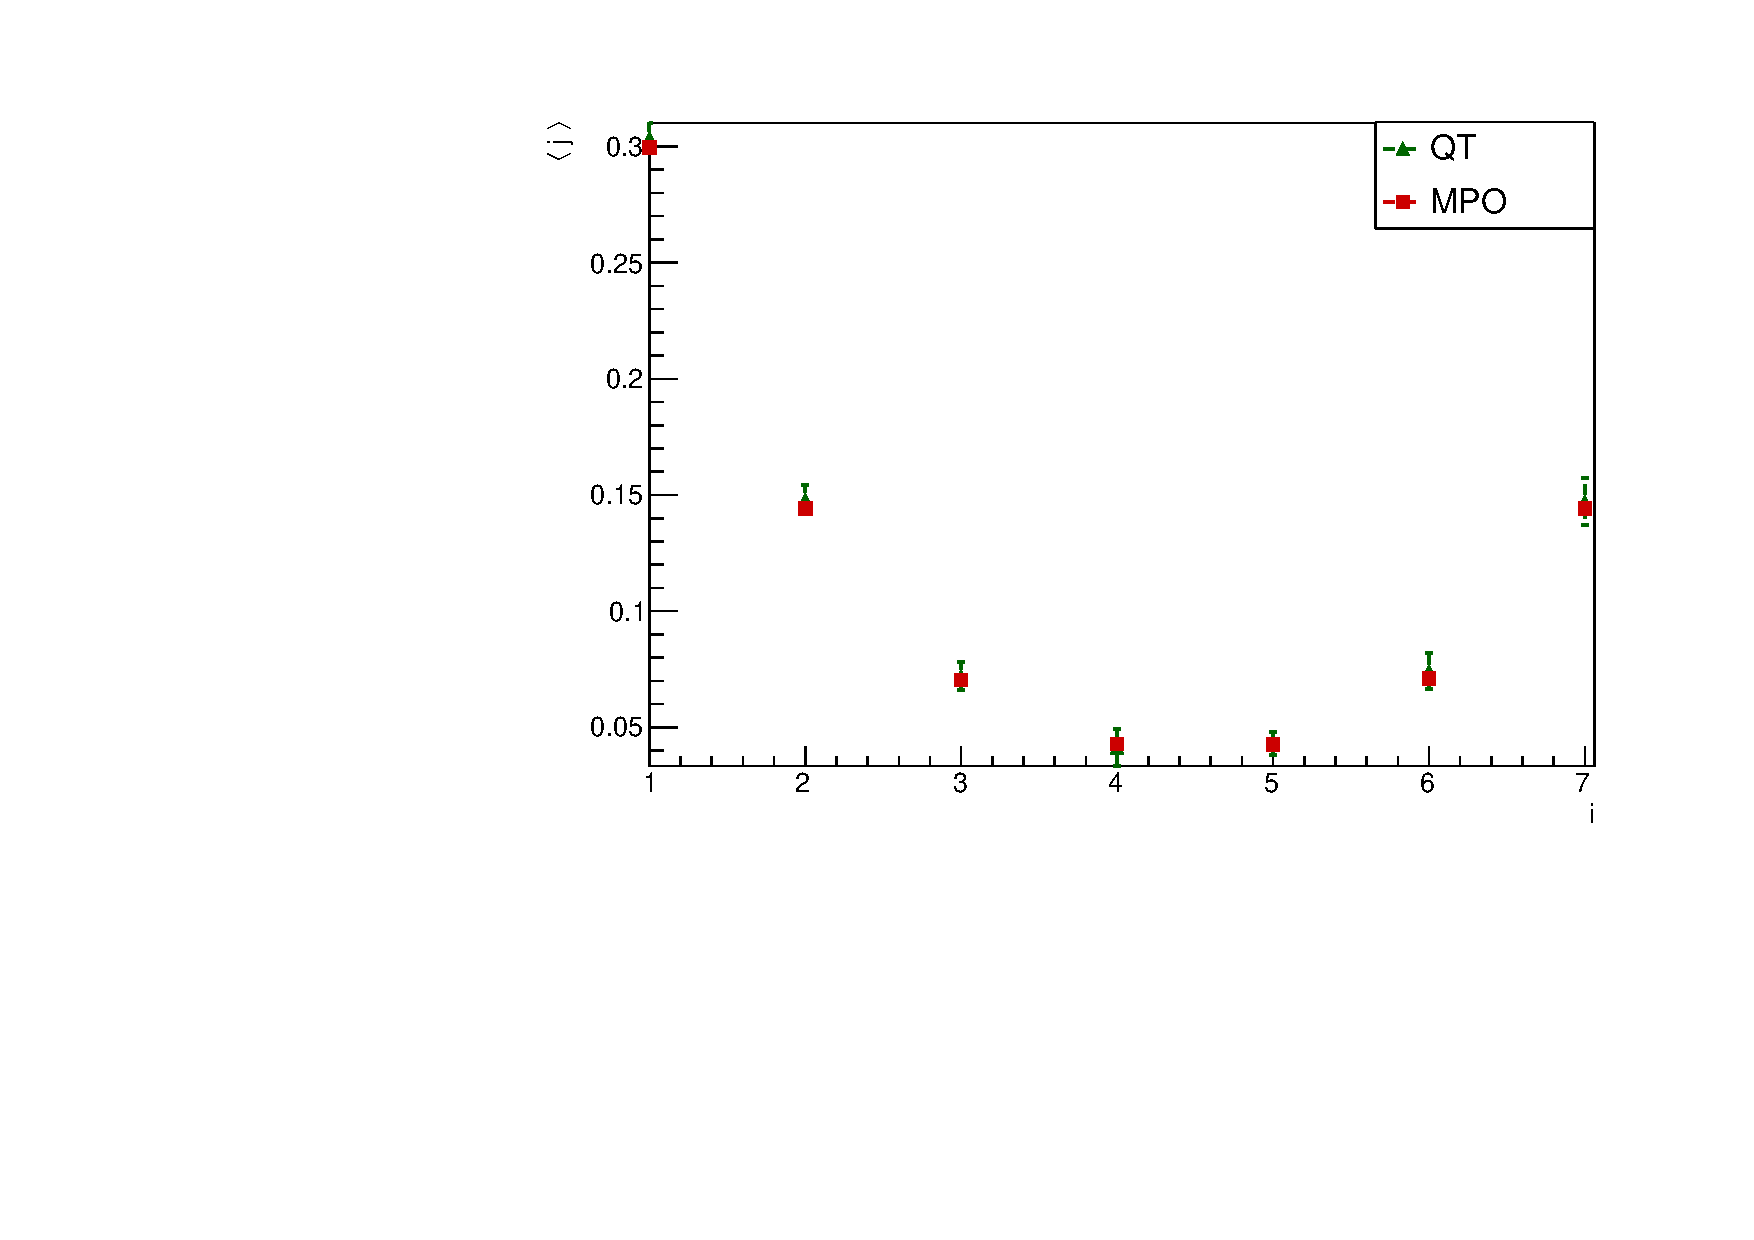
\includegraphics[scale=0.5]{Figures/SpinCurrComparison_8sJ1051.pdf}
        \label{fig:SpinCurrComparison_8sJ1051}
        \end{subfigure}\\
        \begin{subfigure}{\columnwidth}
        \centering
        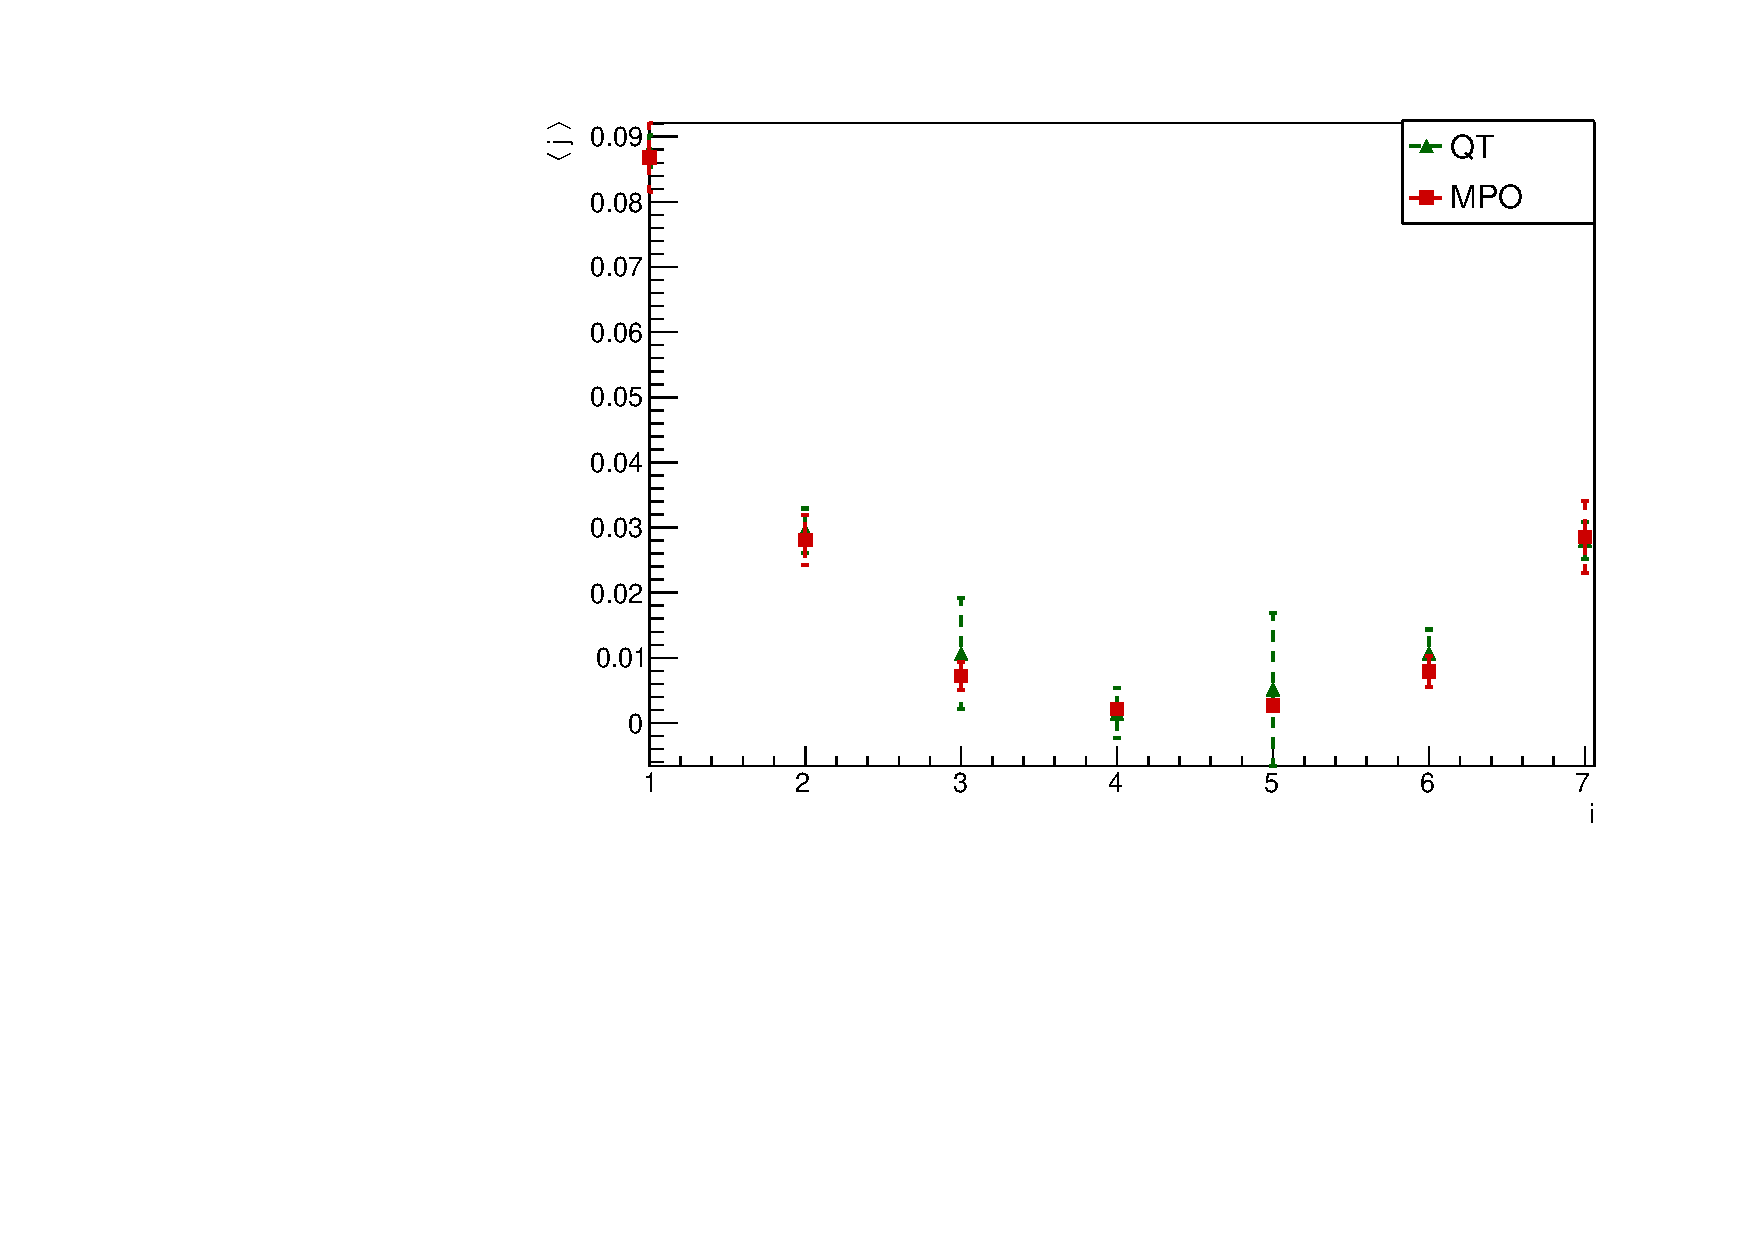
\includegraphics[scale=0.5]{Figures/SpinCurrComparison_8sJ10515.pdf}
        \label{fig:SpinCurrComparison_8sJ10515}
        \end{subfigure}\\
    \caption{Caption}
    \label{fig:my_label}
\end{figure}